\begin{frame}{Método BiLi}
	\begin{columns}
		\column{.9\textwidth}
        \begin{figure}[!hb]
            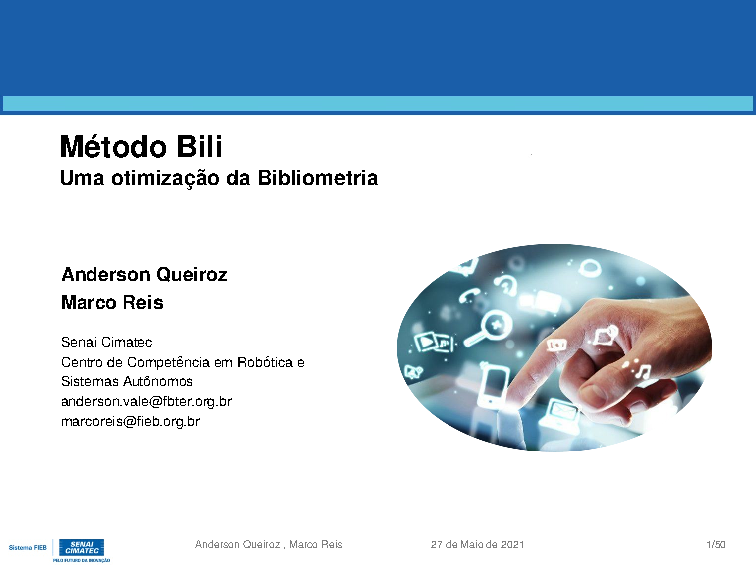
\includegraphics[width=1\textwidth]{figures/bili.png}
        \end{figure}
		\column{.1\textwidth}
		\begin{figure}[hb]
            \includegraphics[width=1.3\textwidth]{figures/ferramentas.png}
		\end{figure}
	\end{columns}
\end{frame}

\begin{frame}{Pré-Requisito}
	\begin{itemize}
		\item Ter instalado o R $\geq$ 3.5
		\begin{itemize}
			\item Windows - https://cran.r-project.org/bin/windows/base/old/3.5.0/
			\item  Ubuntu 18.04 - https://rtask.thinkr.fr/installation-of-r-3-5-on-ubuntu-18-04-lts-and-tips-for-spatial-packages/
		\end{itemize}
		\item Dentro do Console do R instalar:
		\begin{itemize}
			\item Bibliometrix - install.packages(bibliometrix)
			\item LitSearchR - remotes::install\_github("elizagrames/litsearchr", ref="main")
			\item RevTools - install.packages(revtools)
		\end{itemize}
	\end{itemize}
\end{frame}

\begin{frame}{1º Ciclo}

	\begin{columns}
		\column{.5\textwidth}
        Ciclo Ingênuo
		\column{.5\textwidth}
		\begin{figure}[hb]
            \includegraphics[width=0.7\textwidth]{figures/ciclo1.png}
		\end{figure}
	\end{columns}
\end{frame}

\begin{frame}{1º Ciclo - Busca}
	\begin{columns}
		\column{.4\textwidth}
        Fazer uma busca em uma base acadêmica e exportar .bib
        \begin{itemize}
            \item Web Of Science
            \item Scopus
            \item Dimension
            \item PubMed
            \item Cochrane Library
        \end{itemize}
		\column{.6\textwidth}
		\begin{figure}[hb]
            \includegraphics[width=0.9\textwidth]{figures/bases.png}
		\end{figure}
	\end{columns}
\end{frame}

\begin{frame}{1º Ciclo - Bibliometrix}
	Abrir o Bibliometrix no R
	\begin{columns}
		\column{.5\textwidth}
		\begin{figure}[hb]
			\includegraphics[width=1\textwidth]{figures/bibliometrix/rbibliometrix.png}
		\end{figure}
		\column{.5\textwidth}
		\begin{figure}[hb]
			\includegraphics[width=1\textwidth]{figures/bibliometrix/b1.png}
		\end{figure}
	\end{columns}
\end{frame}

\begin{frame}{1º Ciclo - Bibliometrix}
	Importar o .bib
	\begin{columns}
		\column{.5\textwidth}
		\begin{figure}[hb]
			\includegraphics[width=1\textwidth]{figures/bibliometrix/b2.png}
		\end{figure}
		\column{.5\textwidth}
		\begin{figure}[hb]
			\includegraphics[width=0.6\textwidth]{figures/bibliometrix/b3.png}
		\end{figure}
	\end{columns}
\end{frame}

\begin{frame}{1º Ciclo - Bibliometrix}
	Visualização dos dados importados
	\begin{figure}[hb]
		\includegraphics[width=1\textwidth]{figures/bibliometrix/b4.png}
	\end{figure}
\end{frame}

\begin{frame}{1º Ciclo - Bibliometrix}

	Analisar o Co-Citation Network
	\begin{figure}[hb]
		\includegraphics[width=1\textwidth]{figures/bibliometrix/b7.png}
	\end{figure}
\end{frame}

\begin{frame}{1º Ciclo - Bibliometrix}

	Analisar o Co-Citation Network
	\begin{figure}[hb]
		\includegraphics[width=0.9\textwidth]{figures/bibliometrix/b9.png}
	\end{figure}
\end{frame}

\begin{frame}{1º Ciclo - Bibliometrix}

	Analisar o Co-Citation Network
	
	\begin{figure}[hb]
		\centering
		\includegraphics[width=0.6\textwidth]{figures/bibliometrix/brede1.png}
	\end{figure}
	
\end{frame}

\begin{frame}{1º Ciclo - Bibliometrix}

	Analisar o Annual Scientific Production
	
	\begin{figure}[hb]
		\centering
		\includegraphics[width=0.9\textwidth]{figures/bibliometrix/b10.png}
	\end{figure}
	
\end{frame}

\begin{frame}{1º Ciclo - Bibliometrix}

	Analisar o Historiagraph
	
	\begin{figure}[hb]
		\centering
		\includegraphics[width=0.9\textwidth]{figures/bibliometrix/b11.png}
	\end{figure}
	
\end{frame}

\begin{frame}{1º Ciclo - Bibliometrix}

	Analisar o WorldCloud
	
	\begin{figure}[hb]
		\centering
		\includegraphics[width=0.9\textwidth]{figures/bibliometrix/b12.png}
	\end{figure}
	
\end{frame}

\begin{frame}{1º Ciclo - Bibliometrix}

	Analisar o WorldCloud
	\begin{figure}[hb]
		\centering
		\includegraphics[width=0.9\textwidth]{figures/bibliometrix/b13.png}
	\end{figure}
	
\end{frame}

\begin{frame}{1º Ciclo - Bibliometrix}

	Analisar o WorldCloud
	\begin{figure}[hb]
		\centering
		\includegraphics[width=0.9\textwidth]{figures/bibliometrix/b14.png}
	\end{figure}
	
\end{frame}

\begin{frame}{1º Ciclo}

	\begin{columns}
		\column{.3\textwidth}
        Ciclo Ingênuo
		\column{.7\textwidth}
		\begin{figure}[hb]
            \includegraphics[width=0.5\textwidth]{figures/ciclo1.png}
		\end{figure}
	\end{columns}
\end{frame}

\begin{frame}{1º Ciclo - LitSearchR}
	É um pacote R para facilitar o desenvolvimento de estratégia de busca quase automática para revisões sistemáticas.
	\begin{figure}[hb]
		\includegraphics[width=0.9\textwidth]{figures/litsearchr/l1.png}
	\end{figure}
\end{frame}

\begin{frame}{1º Ciclo - LitSearchR}
	\begin{columns}
		\column{.5\textwidth}
		Retorna um novo texto de busca
		\begin{figure}[hb] 
			\includegraphics[width=1.1\textwidth]{figures/litsearchr/l4.png}
		\end{figure}

		\column{.5\textwidth}
		\begin{figure}[hb]
			\includegraphics[width=1\textwidth]{figures/litsearchr/l2.png}
		\end{figure}
		\begin{figure}[!ht]
			\includegraphics[width=1\textwidth]{figures/litsearchr/l3.png}
		\end{figure}
	\end{columns}
\end{frame}

\begin{frame}{1º Ciclo - LitSearchR}
	Refinar palavras chaves
	\begin{figure}[!ht]
		\includegraphics[width=1\textwidth]{figures/litsearchr/l5.png}
	\end{figure}
\end{frame}